\documentclass[conference]{IEEEtran}
\IEEEoverridecommandlockouts
% The preceding line is only needed to identify funding in the first footnote. If that is unneeded, please comment it out.
\usepackage{cite}
\usepackage{amsmath,amssymb,amsfonts}
\usepackage{algorithmic}
\usepackage{graphicx}
\usepackage{textcomp}
\usepackage{xcolor}
\usepackage{float}
\usepackage{caption}
\usepackage{fancyhdr}
\usepackage{lastpage}

\captionsetup[figure]{name=Gambar}
\pagestyle{fancy}
\fancyhf{}
\fancyfoot[C]{\thepage}
\renewcommand{\headrulewidth}{0pt}
\renewcommand{\footrulewidth}{0.4pt}




\def\BibTeX{{\rm B\kern-.05em{\sc i\kern-.025em b}\kern-.08em
    T\kern-.1667em\lower.7ex\hbox{E}\kern-.125emX}}
\begin{document}
\setcounter{page}{1}
\title{Analisis \textit{Fuzzy Time Series}: Mengungkap Pola Harga Singkong}

\author{\IEEEauthorblockN{1\textsuperscript{st} Agus Fuad Mudhofar}
\IEEEauthorblockA{\textit{Departemen Teknik Komputer} \\
\textit{Institut Teknologi Sepuluh Nopember}\\
Surabaya, Indonesia \\
agusfuad090@gmail.com}
\and
\IEEEauthorblockN{2\textsuperscript{nd} Zadun Nafiq}
\IEEEauthorblockA{\textit{Departemen Teknik Komputer} \\
\textit{name of organization (of Aff.)}\\
City, Country \\
email address or ORCID}
\and
\IEEEauthorblockN{3\textsuperscript{rd} Given Name Surname}
\IEEEauthorblockA{\textit{dept. name of organization (of Aff.)} \\
\textit{name of organization (of Aff.)}\\
City, Country \\
email address or ORCID}
\and
\IEEEauthorblockN{4\textsuperscript{th} Given Name Surname}
\IEEEauthorblockA{\textit{dept. name of organization (of Aff.)} \\
\textit{name of organization (of Aff.)}\\
City, Country \\
email address or ORCID}
\and
\IEEEauthorblockN{5\textsuperscript{th} Given Name Surname}
\IEEEauthorblockA{\textit{dept. name of organization (of Aff.)} \\
\textit{name of organization (of Aff.)}\\
City, Country \\
email address or ORCID}
\and
\IEEEauthorblockN{6\textsuperscript{th} Given Name Surname}
\IEEEauthorblockA{\textit{dept. name of organization (of Aff.)} \\
\textit{name of organization (of Aff.)}\\
City, Country \\
email address or ORCID}
}

\maketitle

\begin{abstract}
    Penelitian ini berfokus pada prediksi harga singkong di Indonesia menggunakan metode \textit{Fuzzy Time Series} (FTS). Harga singkong dipengaruhi oleh berbagai faktor seperti kondisi cuaca, permintaan pasar, kebijakan pemerintah, dan biaya produksi, yang dapat menyebabkan variabilitas harga dan berdampak pada pendapatan petani serta stabilitas ekonomi sektor pertanian. Data harga singkong bulanan dari tujuh provinsi di Indonesia selama periode 2020-2022 digunakan untuk membangun model FTS. Proses peramalan melibatkan beberapa langkah, yaitu menentukan interval data, memperoleh data historis, mendefinisikan \textit{fuzzy sets}, membangun hubungan logika \textit{fuzzy}, mencari pola hubungan antar data, dan melakukan peramalan. Hasil peramalan menunjukkan bahwa model FTS dapat memberikan estimasi harga singkong untuk bulan selanjutnya dengan tingkat kesalahan sebesar 2,45\% berdasarkan evaluasi menggunakan \textit{Mean Absolute Percentage Error} (MAPE). Model ini dapat digunakan sebagai alat bantu dalam perencanaan dan pengambilan keputusan di sektor pertanian, meskipun harus selalu diperbarui dengan data terbaru untuk meningkatkan akurasi.
\end{abstract}

\begin{IEEEkeywords}
\textit{Fuzzy Time Series}, Harga Singkong, Prediksi Harga
\end{IEEEkeywords}

\thispagestyle{fancy}
\fancyhf{}
\fancyfoot[C]{\thepage}
\renewcommand{\headrulewidth}{0pt}
\renewcommand{\footrulewidth}{0.4pt}
\section{Pendahuluan}
Indonesia merupakan salah satu negara yang sebagian besar penduduknya bermata pencaharian di bidang pertanian atau bercocok tanam[1]. Dan singkong merupakan salah satu komoditas pertanian yang memiliki peran penting dalam perekonomian banyak negara, termasuk Indonesia. Sebagai bahan pangan, singkong digunakan dalam berbagai produk makanan, pakan ternak, dan industri.  Harga singkong dapat dipengaruhi oleh berbagai faktor seperti kondisi cuaca [2], permintaan pasar, kebijakan pemerintah, dan biaya produksi. Variabilitas harga ini tidak hanya mempengaruhi pendapatan petani tetapi juga berdampak pada stabilitas ekonomi di sektor pertanian.

Dalam menghadapi tantangan ini, prediksi harga singkong dapat menjadi alat untuk memperkirakan harga beberapa bulan kedepan. \textit{Fuzzy Time Series} (FTS) adalah salah satu metode yang menawarkan keunggulan memprediksi data berbasis waktu yang bersifat luas dan dapat digunakan dalam data \textit{realtime}[3]. Penelitian ini bertujuan untuk mengungkap pola harga singkong menggunakan pendekatan Fuzzy Time Series dan mengembangkan model prediksi yang lebih akurat dan dapat diandalkan. Dengan model prediksi yang lebih baik, diharapkan dapat memberikan manfaat signifikan bagi petani, pedagang, dan pembuat kebijakan dalam merencanakan dan mengambil keputusan yang lebih baik.

Melalui analisis ini, penelitian ini tidak hanya berkontribusi pada pengembangan ilmu pengetahuan dalam bidang prediksi harga komoditas tetapi juga berpotensi meningkatkan stabilitas ekonomi sektor pertanian dengan menyediakan alat prediksi yang lebih efektif.


\section{Tinjauan Pustaka}

\subsection{\textit{Fuzzy Time Series}}
\textit{Fuzzy Time Series} (FTS) adalah metode peramalan yang pertama kali dikembangkan oleh Song dan Chissom pada tahun 1993 [4]. Mereka memperkenalkan FTS dalam upaya untuk memprediksi jumlah pendaftaran mahasiswa baru di Universitas Alabama. Sejak awal pengembangannya, FTS telah terbukti efektif dan fleksibel, sehingga diaplikasikan pada berbagai macam masalah peramalan lainnya. Beberapa contoh penerapan FTS termasuk peramalan penjualan, peramalan harga saham, dan peramalan tingkat polusi udara.

FTS menggunakan tiga prinsip utama dalam proses peramalan, yaitu Fuzzifikasi, Hubungan Logika Fuzzy (\textit{Fuzzy Logical Relationship}), dan Peramalan (\textit{Forecasting}). Fuzzifikasi adalah proses mengubah data numerik menjadi data \textit{fuzzy}, yaitu data yang diwakili oleh himpunan \textit{fuzzy}. Setelah data difuzzifikasi, langkah selanjutnya adalah membangun hubungan logika \textit{fuzzy}. Hubungan ini menggambarkan pola hubungan antar nilai data yang telah difuzzifikasi. Terakhir, berdasarkan hubungan logika \textit{fuzzy} yang telah dibangun, dilakukan peramalan untuk memprediksi nilai data di masa depan.

Secara lengkap, proses peramalan menggunakan FTS terdiri dari beberapa tahapan, yaitu:
\begin{enumerate}
    \item Menentukan interval data dan jumlah himpunan \textit{fuzzy}
    \item Memperoleh data historis
    \item Mendefinisikan \textit{fuzzy sets} berdasarkan interval data dan data historis
    \item Membangun hubungan logika \textit{fuzzy}
    \item Mencari pola hubungan antar data
    \item Memasukan data input kedalam model FTS dan melakukan peramalan
\end{enumerate}


\section{Metode Penelitian}

Penelitian ini menggunakan data harga singkong dari tahun 2020 hingga 2022. Data ini diperoleh dari hasil laporan yang diterbitkan oleh Kementerian Pertanian Indonesia yang bekerja sama dengan Badan Pusat Statistik. Data yang digunakan adalah data bulanan yang mewakili banyak wilayah di Indonesia dengan didasarkan kepada 7 provinsi yaitu Lampung, Jawa Tengah, Jawa Timur, Jawa Barat, Sumatera Utara, Yogyakarta, dan NTT. Data ini kemudian diolah dan dianalisis menggunakan metode Fuzzy Time Series dengan diagram \textit{flowchart} sebagai berikut:

\begin{figure}[htbp]
    \centering
    {\includegraphics[scale=0.7]{flowchart.png}} 
    \caption{\textit{Flowchart} Pengolahan Data}
\end{figure}


\subsection{Menentukan interval data dan jumlah himpunan \textit{fuzzy}}\label{AA}
Untuk menentukan interval data dan jumlah himpunan \textit{fuzzy} yang tepat, disini digunakan rumus Sturges sebagai berikut:
\begin{equation}
    k = 1 + 3.33 \times \log_{10}(n)
\end{equation}
dimana $k$ adalah jumlah kelas, dan $n$ adalah jumlah data. Data yang digunakan adalah data harga singkong dari tahun 2020 hingga 2022, sehingga $n = 36$. Dengan menggunakan rumus tersebut, didapatkan $k = 6.1$. Karena jumlah kelas harus berupa bilangan bulat, maka jumlah kelas yang digunakan adalah 6.
\subsection{Memperoleh data historis}
Data historis yang digunakan adalah data harga singkong dari tahun 2020 hingga 2022. Data ini diperoleh dari hasil laporan yang diterbitkan oleh Kementerian Pertanian Indonesia yang bekerja sama dengan Badan Pusat Statistik. Data yang digunakan adalah data bulanan yang mewakili banyak wilayah di Indonesia dengan didasarkan kepada 7 provinsi yaitu Lampung, Jawa Tengah, Jawa Timur, Jawa Barat, Sumatera Utara, Yogyakarta, dan NTT.

\begin{figure}[H]
    \centering
    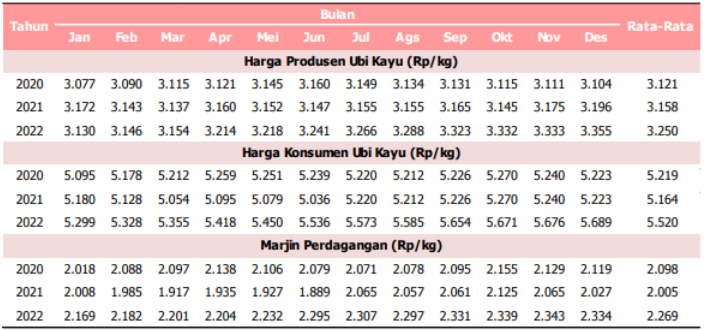
\includegraphics[scale=0.5]{images/Data Historis.png} 
    \caption{Data Historis Harga Singkong}
\end{figure}
Data harga yang digunakan dalam penelitian ini adalah data harga singkong produsen dari tahun 2020 hingga 2022. Data ini kemudian diolah dan dianalisis menggunakan metode Fuzzy Time Series untuk memprediksi harga singkong di bulan selanjutnya.

\subsection{Mendefinisikan \textit{fuzzy sets} berdasarkan interval data dan data historis}
Dalam mendefinisikan \textit{fuzzy sets}, digunakan pengelompokkan berdasarkan interval data. Metode ini membagi data menjadi beberapa interval berdasarkan rentang nilai data. Setiap interval kemudian diwakili oleh himpunan \textit{fuzzy}. Dalam penelitian ini, digunakan 6 interval data yang masing-masing diwakili oleh himpunan \textit{fuzzy}, yaitu:
\begin{figure}[H]
    \centering
    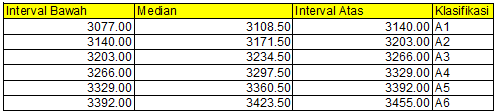
\includegraphics[scale=0.7]{images/Fuzzifikasi.png} 
    \caption{Fuzzifikasi}
\end{figure}

\subsection{Membangun hubungan logika \textit{fuzzy}}
Dalam membangun hubungan logika \textit{fuzzy}, digunakan metode Fuzzy Logical Relationship (FLR). Metode ini membangun hubungan antar data dengan menggunakan aturan \textit{fuzzy}. Aturan ini menggambarkan pola hubungan antar data yang telah difuzzifikasi. Metode ini akan memapping klasifikasi data harga bulan ini ke dalam klasifikasi data harga bulan selanjutnya. Dengan hasil mapping sebagai berikut:
\begin{figure}[H]
    \centering
    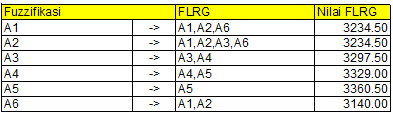
\includegraphics[scale=0.7]{images/FLR.png} 
    \caption{Fuzzy Logical Relationship}
\end{figure}
Nilai FLRG adalah nilai yang didapat dari hasil mapping antara data harga bulan ini dengan data harga bulan selanjutnya. Nilai ini digunakan untuk memprediksi harga singkong di bulan selanjutnya.
Untuk mendapatkan nilai FLRG, digunakan rumus sebagai berikut:
    \begin{equation}
        FLRG = \frac{\text{Median (FLRG)}}{n}
    \end{equation}
    \begin{equation*}
        FLRG_{A1} = \frac{3108.5 + 3171.5 + 3423.5}{3}
    \end{equation*}
    \begin{equation*}
        FLRG_{A1} = 3234.5
    \end{equation*}
   



\subsection{Mencari pola hubungan antar data}
Langkah selanjutnya adalah mencari pola hubungan antar data pada data yang telah diperoleh. Dengan menggunakan metode FTS, didapatkan pola hubungan antar data sebagai berikut:
\begin{figure}[H]
    \centering
    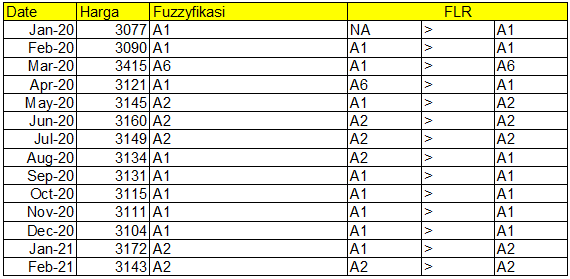
\includegraphics[scale=0.5]{images/Pola data.png} 
    \caption{Pola Hubungan Antar Data}
\end{figure}
Data diatas merupakan hasil dari pencarian pola hubungan antar data yang dilakukan dengan menggunakan metode FTS. Data ini diambil sebagian saja sebagai contoh visualisasi pola hubungan antar data.



\subsection{Memasukan data input kedalam model FTS dan melakukan peramalan}
Langkah terakhir adalah memasukan data input kedalam model FTS dan melakukan peramalan. Dengan menggunakan data historis yang telah diperoleh, data input dimasukan kedalam model FTS. Model ini kemudian melakukan peramalan untuk memprediksi harga singkong di bulan selanjutnya. Hasil peramalan ini kemudian digunakan sebagai dasar untuk membuat keputusan yang lebih baik dalam merencanakan dan mengelola harga singkong. Berikut adalah contoh hasil peramalan harga singkong menggunakan model FTS:
\begin{figure}[H]
    \centering
    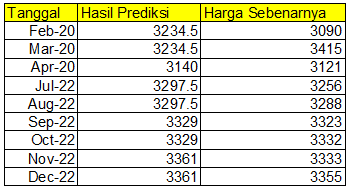
\includegraphics[scale=0.5]{images/Peramalan.png} 
    \caption{Peramalan Harga Singkong}
\end{figure}
Dengan menggunakan model FTS, didapatkan hasil peramalan harga singkong untuk bulan selanjutnya. Hasil ini dapat menjadi perkiraan harga singkong di bulan selanjutnya. Peramalan harga singkong ini harus selalu diperbarui dengan data terbaru untuk mendapatkan hasil yang lebih akurat dan dapat diandalkan karena jika mengandalkan pola harga yang sudah lama, maka hasil peramalan akan kurang akurat.

\subsection{Evaluasi Model}
Evaluasi model dilakukan dengan membandingkan hasil peramalan dengan data aktual. Dengan menggunakan metode \textit{Mean Absolute Percentage Error} (MAPE), dapat dihitung tingkat kesalahan peramalan. MAPE adalah metode yang digunakan untuk mengukur tingkat kesalahan peramalan dengan cara menghitung rata-rata persentase kesalahan peramalan[5]. Rumus MAPE adalah sebagai berikut:
\begin{equation}
    MAPE = \frac{1}{n} \sum_{t=1}^{n} \left| \frac{A_t - F_t}{A_t} \right| \times 100\%
\end{equation}
dimana $A_t$ adalah data aktual, $F_t$ adalah data peramalan, dan $n$ adalah jumlah data. Dengan menggunakan rumus tersebut, dapat dihitung tingkat kesalahan peramalan dan mengevaluasi model yang telah dibangun. Berdasrkan hasil evaluasi, model FTS dalam penelitian ini memiliki tingkat kesalahan sebesar 2.45\% yang menunjukkan bahwa model ini cukup akurat dan dapat diandalkan untuk memprediksi harga singkong di bulan selanjutnya.



\section{Hasil dan Pembahasan}
Dari hasil pengolahan data yang telah dilakukan didapat data prediksi harga singkong untuk bulan Januari 2023 adalah Rp 3.361,00. Data ini dihasilkan dari model FTS yang telah dibangun berdasarkan data historis harga singkong dari tahun 2020 hingga 2022.
Fuzzy Time Series (FTS) kurang cocok digunakan untuk memprediksi data yang memerlukan keakuratan yang sangat tinggi dan tingkat ketelitian yang tinggi. FTS lebih cocok digunakan untuk memprediksi data yang bersifat luas dan tidak memerlukan keakuratan yang sangat tinggi. Oleh karena itu, model FTS yang telah dibangun dalam penelitian ini dapat digunakan sebagai alat bantu untuk memprediksi harga singkong di bulan selanjutnya. Namun, model ini harus selalu diperbarui dengan data terbaru untuk mendapatkan hasil yang lebih akurat dan dapat diandalkan.



\begin{thebibliography}{00}
\bibitem{b1} Sarbaini, S., \& Yanti, D. (2023). Prediksi Harga Beras Belida Di Kota Pekanbaru Menggunakan Fuzzy Time Series Cheng. Jurnal Teknologi dan Manajemen Industri Terapan, 2(3), 234-241.
\bibitem{b2}Kementerian Pertanian. (2023). Pengaruh Perubahan Iklim Terhadap Sektor Pertanian. Upland.psp.pertanian.go.id. Diakses pada 15 Juni 2024, dari https://upland.psp.pertanian.go.id/public/artikel/1687919315/pengaruh-perubahan-iklim-terhadap-sektor-pertanian
\bibitem{b3} Ikhsanudin, A., Santoso, K. I., \& Wahyudion, S. (2022). Metode Fuzzy Time Series Model Chen untuk Memprediksi Jumlah Kasus Aktif Covid-19 di Indonesia. TRANSFORMASI, 18(1).
\bibitem{b4} Sumartini, S., Hayati, M. N., \& Wahyuningsih, S. (2017). Peramalan Menggunakan Metode Fuzzy Time Series Cheng. EKSPONENSIAL, 8(1), 51-56.
\bibitem{b5} Murni, C. K. (2023). Perbandingan Peramalan Penjualan Minuman Menggunakan Algoritma Single Exponential Smoothing Dan Triple Exponential Smoothing. Journal of Informatics Development, 1(2), 59-64.
\end{thebibliography}

\end{document}